\chapter{Parameter Inference}

\section{Motivation}

Building mathematical models of real world phenomenon allows for us to
simulate changes in the world without having to undertake large scale
experiments. However, once we have a model that sufficiently approximates
\emph{P. vivax} transmission
or anything else we are trying to model,
we then need to estimate what the `true' underlying parameters are.
To do this we calibrate the model against real world data such as case counts,
and prevalence surveys. Under frequentist assumptions, there is a `true' set of
parameters that if used in our model, simulated the observed data. Under a Bayesian 
assumption, the parameters are considered to be random, and
This chapter explores statistical inference techniques to recover the 
parameters, under both the frequentist and Bayesian frameworks.

\section{Frequentist Parameter Estimation}

Assume the model is parametrised by a set of parameters
$\btheta \in \mathbf{\Theta}$ which
we are trying to estimate by considering some observed data
$\mathbf{y}^\obs = (y_1^\obs, \dots, y_n^\obs).$
Consider $\mathbf{f}(\btheta) = (f_1(\btheta), \dots, f_n(\btheta))$
some model simulation of
$\mathbf{y}^\obs.$ Often the observed data has some underlying index set
$x_1, \dots, x_n,$ where $x_i$ might be something like time. In this case
we can also consider the observed data to be
$\{(x_1, y_1^\obs), \dots, (x_n, y_n^\obs)\},$ and the
model simulated data to be
$\{(x_1, f_1(\btheta)), \dots, (x_n, f_n(\btheta))\}.$

\subsection*{Least Squares Estimator}

It is common that models are not random, but instead model the mean behaviour
of a system. In this case, $\mathbf{f}(\btheta)$ is not random. Therefore
we can assume that $y^\obs_i = f_i(\btheta) + \varepsilon_i,$
where $\varepsilon_i$ is a random variable with some (possibly unknown)
distribution, and zero mean.

When the distribution of $\varepsilon_i$ is unknown, a common approach for
estimating $\btheta^{\LS}$ is to take the least squares estimate.

\begin{definition}[Least Squares Estimate]
    The \emph{least squares estimate} $\btheta^{\LS}$ for
    $\btheta$ is
    $$
        \btheta^{\LS}
        := \argmin_{\btheta\in\mathbf{\Theta}}
        \sum_{i = 1}^n (f_i(\btheta)- y_i^\obs)^2.
    $$
\end{definition}

\begin{example}\label{ex:LSE}
    Consider the observed data
    $\{(x_1, y_1^\obs), (x_2, y_2^\obs), (x_3, y_3^\obs)\}
        = \{(1, 2), (2, 4), (3, 4)\},$
    which we assume were generated from the model
    $f_i(\btheta) + \varepsilon_i,$ where
    $f_i(\btheta) = \theta_0 + \theta_1x_i,$ and
    $\E(\varepsilon_i) = 0.$ We derive the least squares estimate of our
    parameters $\btheta = (\theta_0, \theta_1)$ by

    \begin{align*}
        \btheta^{\LS}
        = & \, \argmin_{\btheta}
        [\sum_{i = 1}^3 (f_i(\btheta) - y_i^\obs)^2]           \\
        = & \, \argmin_{\btheta}
        [\sum_{i = 1}^3 (\theta_0 + \theta_1x_i - y_i^\obs)^2] \\
        = & \, \argmin_{\btheta}
        [(\theta_0 + \theta_1 - 2)^2 + (\theta_0 + 2\theta_1 - 4)^2
            + (\theta_0 + 3\theta_1 - 4)^2]
    \end{align*}

    Since the expanded quadratic will have positive coefficients out the front
    of $\theta_0$ and $\theta_1,$ we can solve for $\btheta^{\LS}$
    by

    \begin{align*}
        \mathbf{0}
        = & \, \frac{\partial}{\partial \btheta}
        [
            (\theta^\LS_0 + \theta^\LS_1 - 2)^2
            + (\theta^\LS_0 + 2\theta^\LS_1 - 4)^2
            + (\theta^\LS_0 + 3\theta^\LS_1 - 4)^2
        ]                                        \\
        = & \begin{bmatrix}
                6\theta^\LS_0 + 12\theta^\LS_1 - 20 \\
                12\theta^\LS_0 + 28\theta^\LS_1 - 44
            \end{bmatrix}
    \end{align*}
    And solving these two equations results in $\theta^\LS_0 = 4/3$ and
    $\theta^\LS_1 = 1.$ This can be visually seen in Figure \ref{fig:LSE}
\end{example}


\begin{figure}[htbp]
    \centering
    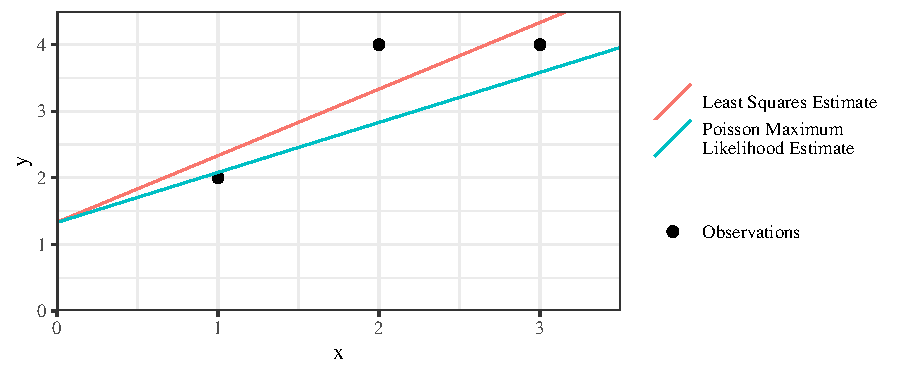
\includegraphics[width=\textwidth]{LS_example.pdf}
    \caption{
        Two linear models of the form
        $f_i(\btheta) = \theta_0 + \theta_1x_i$ fit given the set
        of observations $\{(1, 2), (2, 4), (3, 4)\}$ using the method of
        least squares and maximum likelihood under
        the assumption that the data are independent realisations by a Poisson
        distribution with $\Pois(f_i(\btheta)).$ The least squares estimates
        were $\theta^\LS_0 = 4/3$ and $\theta^\LS_1 = 1.$ The maximum likelihood
        estimates were $\hat{\theta}_0 \approx 1.329$ and
        $\hat{\theta}_1 \approx 0.751.$
    }
    \label{fig:LSE}
\end{figure}

\subsection*{Maximum Likelihood Estimator}

The least square method makes no explicit assumptions about the distribution
of the noise $\varepsilon.$ However if the distribution of $\varepsilon$ is
known (or can be reasonably assumed), we can
explicitly calculate the probability of the data given the parameters.

\begin{definition}[Likelihood function]
    With $\mathbf{y}^\obs$ fixed, the \emph{likelihood function} is
    $$
        \mathcal{L}(\btheta)
        := \Pr(
        \mathbf{f}(\btheta) + \bm{\varepsilon} = \mathbf{y}^\obs
        | \btheta
        ).
    $$
    Particularly, if $f_i(\btheta) + \varepsilon_i$ are independent
    $$
        \mathcal{L}(\btheta)
        = \prod_{i = 1}^n
        \Pr(
        f_i(\btheta) + \varepsilon_i = y_i^\obs
        | \btheta
        ).
    $$
    In the continuous case, if $\mathbf{f}(\btheta) + \bm{\varepsilon}$
    has joint density $g,$
    $$
        \mathcal{L}(\btheta)
        := g(\mathbf{y}^\obs | \btheta).
    $$
\end{definition}

Note that the dependence on $\mathbf{y}^\obs$ is suppressed, but can be
explicitly written as $\mathcal{L}(\btheta|\mathbf{y}^\obs)$
A natural estimate for $\btheta$ is the one that maximises the likelihood
function, as it coincides with the value of $\btheta$ maximises the
probability of the data. Such an estimate is called the maximum likelihood
estimate.

\begin{definition}[Maximum Likelihood Estimate]
    The \emph{maximum likelihood estimate} of $\btheta$ is
    $$
        \hat{\btheta}
        := \argmax_{\btheta\in\mathbf{\Theta}} \mathcal{L}(\btheta)
    $$
\end{definition}

It is often computationally easier to deal with the log-likelihood
$\ell(\btheta) := \ln\mathcal{L}(\btheta).$ Since $\ln$ is a monotonic function,
$\argmax_{\btheta\in\mathbf{\Theta}} \mathcal{L}(\btheta)
    = \argmax_{\btheta\in\mathbf{\Theta}} \ell(\btheta)$

\begin{example}
    Using the same observed data set as Example \ref{ex:LSE}, we assume that
    $y_i^\obs$ were generated independently from
    $f_i(\btheta) + \varepsilon_i \sim \Pois(f_i(\btheta)),$ where
    $f_i(\btheta) = \theta_0 + \theta_1x_i$ as previously defined. Therefore
    the maximimum likelihood estimate of $\btheta$ is
    \begin{align*}
        \hat{\btheta}
        = & \, \argmax \ell(\btheta)                                  \\
        = & \, \argmax_{\btheta\in\mathbf{\Theta}}\sum_{i = 1}^{3}
        y_i^\obs\ln(f_i(\btheta)) -y_i^\obs(\btheta) - \ln(y_i^\obs!) \\
        = & \, \argmax_{\btheta\in\mathbf{\Theta}}\sum_{i = 1}^{3}
        y_i^\obs\ln(\theta_0 + \theta_1x_i)
        - \theta_0 - \theta_1x_i
        - \ln(y_i^\obs!)                                              \\
        = & \, \argmax_{\btheta\in\mathbf{\Theta}}
        2\ln(\theta_0 + \theta_1) - \theta_0 - \theta_1
        + 4\ln(\theta_0 + 2\theta_1) - \theta_0 - 2\theta_1
        + 4\ln(\theta_0 + 3\theta_1) - \theta_0 - 3\theta_1
    \end{align*}
    which we numerically solve to get $\hat{\theta}_0 \approx 1.329$
    and $\hat{\theta_1} \approx 0.751,$ as seen in Figure \ref{fig:LSE}.
\end{example}

\subsection*{Relationship of Least Squares and Maximum Likelihood Estimates}

Although the least squares estimate does not explicitly assume a distribution,
it coincides with the maximum likelihood estimate under the assumption that
the $y_i^\obs$s were has been generated with normal error.

\begin{theorem}
    If $f_i(\btheta) + \epsilon_i \sim N(f_i(\btheta), \sigma^2),$ then
    $$
        \hat{\btheta} = \btheta^\LS
    $$
\end{theorem}

\begin{proof}
    \begin{align*}
        \hat{\btheta}
        = & \, \argmax_{\btheta\in\mathbf{\Theta}}\ell(\btheta) \\
        = & \, \argmax_{\btheta\in\mathbf{\Theta}}
        \sum_{i = 1}^n
        \ln(\frac{1}{\sqrt{2\pi}\sigma})
        -\frac{(f_i(\btheta)- y_i^\obs)^2}{\sigma^2}            \\
        = & \argmax_{\btheta\in\mathbf{\Theta}} \sum_{i = 1}^n
        - \frac{(f_i(\btheta)- y_i^\obs)^2 }{\sigma^2}          \\
        = & \argmax_{\btheta\in\mathbf{\Theta}} \sum_{i = 1}^n
        - (f_i(\btheta)- y_i^\obs)^2                            \\
        = & \argmin_{\btheta\in\mathbf{\Theta}} \sum_{i = 1}^n
        (f_i(\btheta)- y_i^\obs)^2                              \\
        = & \btheta^\LS.
    \end{align*}
\end{proof}

\subsection*{Frequentist Parameter Estimates in Compartmental Models}

Various approaches are possible to parameterise compartmental models.
Often the ODE model is fit to the data directly (if there is only one datapoint)
to fit to, or parameters are estimates by least squares. For example see
\cite{gani_transmission_2001} who use both these methods.
including fitting the ODEs to by using the least squares estimates of
a common approach is to find the least squares 
estimate of the parameters by considering $\mathbf{f}(\btheta).$
This is commonly done because explicitly solving the likelihood for 
the stochastic compartmental model is infeasible. An alternative approach
is to assume that the observed data follow a particular distribution
determined by the ODE solution. For example, for the SIS model described
in \ref{fig:SIS_model} it is plausible to assume that
daily incidence (case counts) are distributed $\Pois(\beta \frac{I_t}{N}S_t).$ 
Then $\beta$ could be estimated using a maximum likelihood estimate given the 
case counts.
Alternatively if case counts are overdispered, a negative binomial likelihood
could be used.

\begin{figure}
    \missingfigure{MLE Poisson SIS model}
\end{figure}